\chapter{Business Understanding}

HousePrice is a tool used for forecasting the selling prices of real estate. When one thinks of a house, from the point of view of the buyers, it is usual to think of purely aesthetic parameters such as a beautiful and large kitchen, a sunny balcony, a guest room without paying much attention to aspects that actually contribute to the price end of the structure, such as the area in which it is located, its proximity to the railway, materials used in the construction, the type of road to access the property, the cadastre of the lot, type of foundations, type of heating, quality of the floors and many other parameters that are generally not considered or are considered as minor. The combination of all these aspects, albeit for some subjects considered of little importance, contribute to a better economic evaluation of the property.



\section{Determine Business Objectives}
Understanding a customer's true goal is as critical for many reasons as understanding the goal you intend to achieve and where to focus your attention in implementation. It is also important to measure the success of the result achieved.

\subsection{Background}
%Record information that is known about the organization’s business situation
Kaggle is an online community of data scientists and machine learning professionals. Enables users to find and publish datasets, explore and build models in a web-based data science environment, work with other data scientists and machine learning engineers, and enter contests to solve data science challenges.

\subsection{Business Objectives}
%(Describe primary objective from a business perspective) 
The goal is to understand which parameters contribute to the market value of a house, which of them allow to increase the economic value more and which less.

\subsection{Business success criteria}
%(Describe the criteria that you’ll see to determine if the project has been successful)
The criterion we use are the relationships that we find between the various attributes that lead to substantial changes in the market value of the house in question.



\section{Assess Situation}
This task involves the resources, requirements, constraints, assumptions, risks, contingencies, glossary of terminology, and the cost-benefit analysis.

\subsection{Inventory of resources}
List of resources available to the project:
\begin{itemize}
\item Personnel: five students of machine learning; 
\item Data: fixed extracts;
\item Computing resources: laptops;
\item Software: Jupyther v.6.4.12. OTHER????
\end{itemize}

\subsection{Requirements, assumptions and constraints}
% List of all requirements of the project, of the assumptions made by the project and list of the constraints on the project
We are not sure that these requirements are the only ones that are relevant in estimating the value of a house, such as the unmentioned plumbing system. Furthermore, the use of new materials on the market, which perhaps have a lower environmental impact but a worse yield than conventional products, are we sure they are evaluated correctly? This of course cannot be verified during data mining nor with any other project-related activity, yet they are worth seeing and mentioning.

\subsection{Risks and contingencies}
\begin{itemize}
\item List of risks or event that might delay the project or cause it to fail: For timing reasons we don't know if we will be able to compare different modeling techniques, in order to find the technique that best describes our problem; 
\item List of actions to be carried out if the risks arises: In case this problem arises, we are satisfied to be able to conclude a correct analysis and estimation of a modeling technique.
\end{itemize}	

\subsection{Terminology}
%Glossary of terminology relevant to the project) (LATER)
\begin{itemize}
\item Extreme programming: it is one of the most famous agile methodologies. It's an extreme of iterative development, where multiple versions can be built multiple times in a day, increments are delivered to customers every two weeks. Developers work in pairs, checking each other's work, giving support to do a good job; 
\item Agile methodology: there is a lot of focus on the code and the product to be delivered as opposed to wasting time on other aspects deemed secondary. The principles of this methodology allow you to create software that works quickly.
\end{itemize}

\subsection{Costs and benefits}
%A cost-benefit analysis which compares the costs of the project with the potential benefits
This project involves a more objective assessment of the property than an assessment, albeit made by a person who has gained some experience, by eye and therefore in a subjective way. Very often, some properties have disproportionate prices as there is no rigid guideline to follow in order to estimate a property but the real estate agencies themselves take care of making estimates according to parameters that are ephemeral compared to those considered by the HousePrice system.



\section{Determine Data Mining Goals}
A business goal states objectives in business terminology while a data mining goal states project objectives in technical terms.

\subsection{Data mining Goals}
%(Describe the intended outputs that enables the achievement of the project objectives) 
The goal is to create a tool capable of estimating new properties that will be put on the market, understanding the importance of the parameters that contribute to the economic evaluation of the property, in order to have a more accurate estimate of the value of the property based on the parameters that allow its value to be surveyed. For each property there is no right or wrong answer to its market value and it is not even possible to make a comparison with other properties present, albeit close to rent, as each property has different characteristics from each other.

\subsection{Data mining Success Criteria}
%(Define the criteria for a successful outcome) 
The criterion we use to determine if our project is successful is to find the best valuation model to rank the final price of each house.



\section{Produce Project Plan}
Description of the plan envisaged to achieve the data mining objectives and thereby achieve the business objectives.

\subsection{Project Plan}
%(List of the stages to be executed, together with their duration, resources required, inputs, outputs and dependencies)

\begin{figure}[t]
    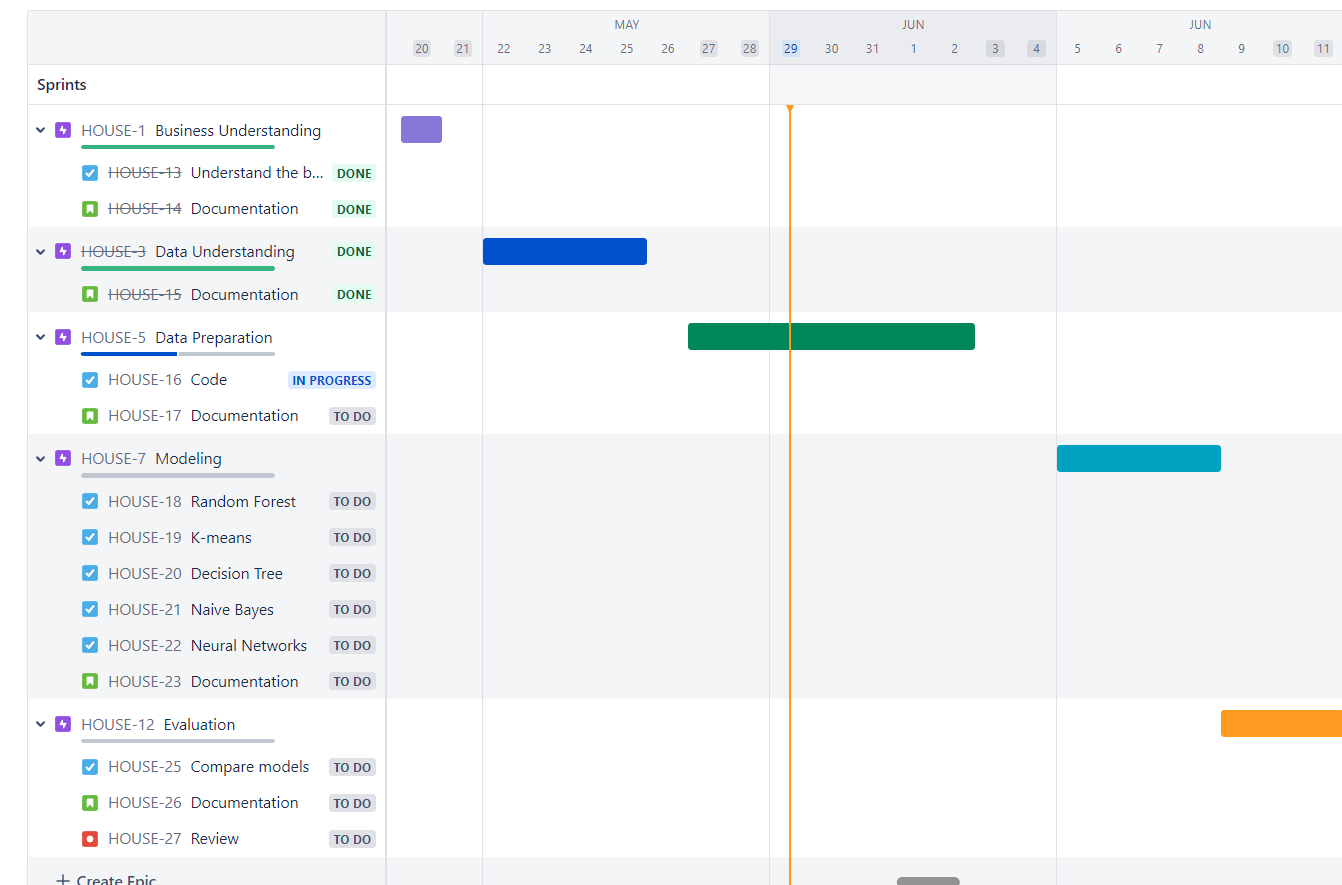
\includegraphics[scale=0.45]{imgs/jira_schedule.png}
    \centering
    \caption{Jira schedule}
    \hrulefill\vspace{15pt}\par
\end{figure}

The phases that we are going to perform by dividing the work by trying different methodologies in order to create a model as close as possible to the training set provided. Initially we plan to work together to get to know each other better, understand the individual potentials of each of us and to understand and respect the objective of the project. Subsequently, let's assume that we can work according to a methodology defined as Extreme Programming.
We plan to spend our time, as is possible see in the figure 1.1, distributing the hours in this way:
\begin{itemize}
\item Business Understanding: 5\% of total hours;
\item Data Understanding: 20\%;
\item Data Preparation: 40\%; 
\item Modeling: 30\%;
\item Evaluation: 10\%.
\end{itemize}

\subsection{Initial Assessment of Tools and
Techniques}
